\chapter[Eletrônica]{Eletrônica}


\section{Requisitos do Projeto}
 
 A construção de uma máquina de venda autômoma de chopp depende da construção de diversos subsistemas,
 que correspondem aos requisitos do projeto. Assim, seguem os requisitos do projeto.

\begin{itemize}
\item Controle de temperatura
\item Controle de saída chopp
\item Atuação de motores
\item Abertura do reservatório de copos
\end{itemize}
  
Os códigos utilizados neste trabalho encontram-se em controle de versão na ferramenta GitHub 
e podem ser facilmente acessados em: \url{https://github.com/autochopp/embedded_electronics}. 

\section{Casos de teste}

\section{Funcionamento}

\section{Solução adotada}

\subsection{Controle de temperatura}

Para realizar o controle da temperatura, permitindo que o chopp esteja sempre gelado quando da retirada, 
foi utilizado o sensor de temperatura DS18B20 presente na Figura \ref{sensor-temperatura} , 
este sensor permite a leitura de temperatura até mesmo em ambientes úmidos, tal qual esta aplicação. 
O sensor descrito mede temperaturas entre   $ -55 ^\circ C$ e $125 ^\circ C$ com erro de $\pm 0.5 ^\circ C$.
O sensor convencionado de ser posicionado na saída de chopp permitindo uma leitura mais fidedigna da
temperatura real do chopp, pois na saída o chopp já circulou por toda a serpentina e estará mais próximo 
do equilíbrio térmico. O modo como esse sensor é conectado pode ser visto na Figura \ref{esquema-temperatura}.

\begin{figure}[!htb]
            \centering
         	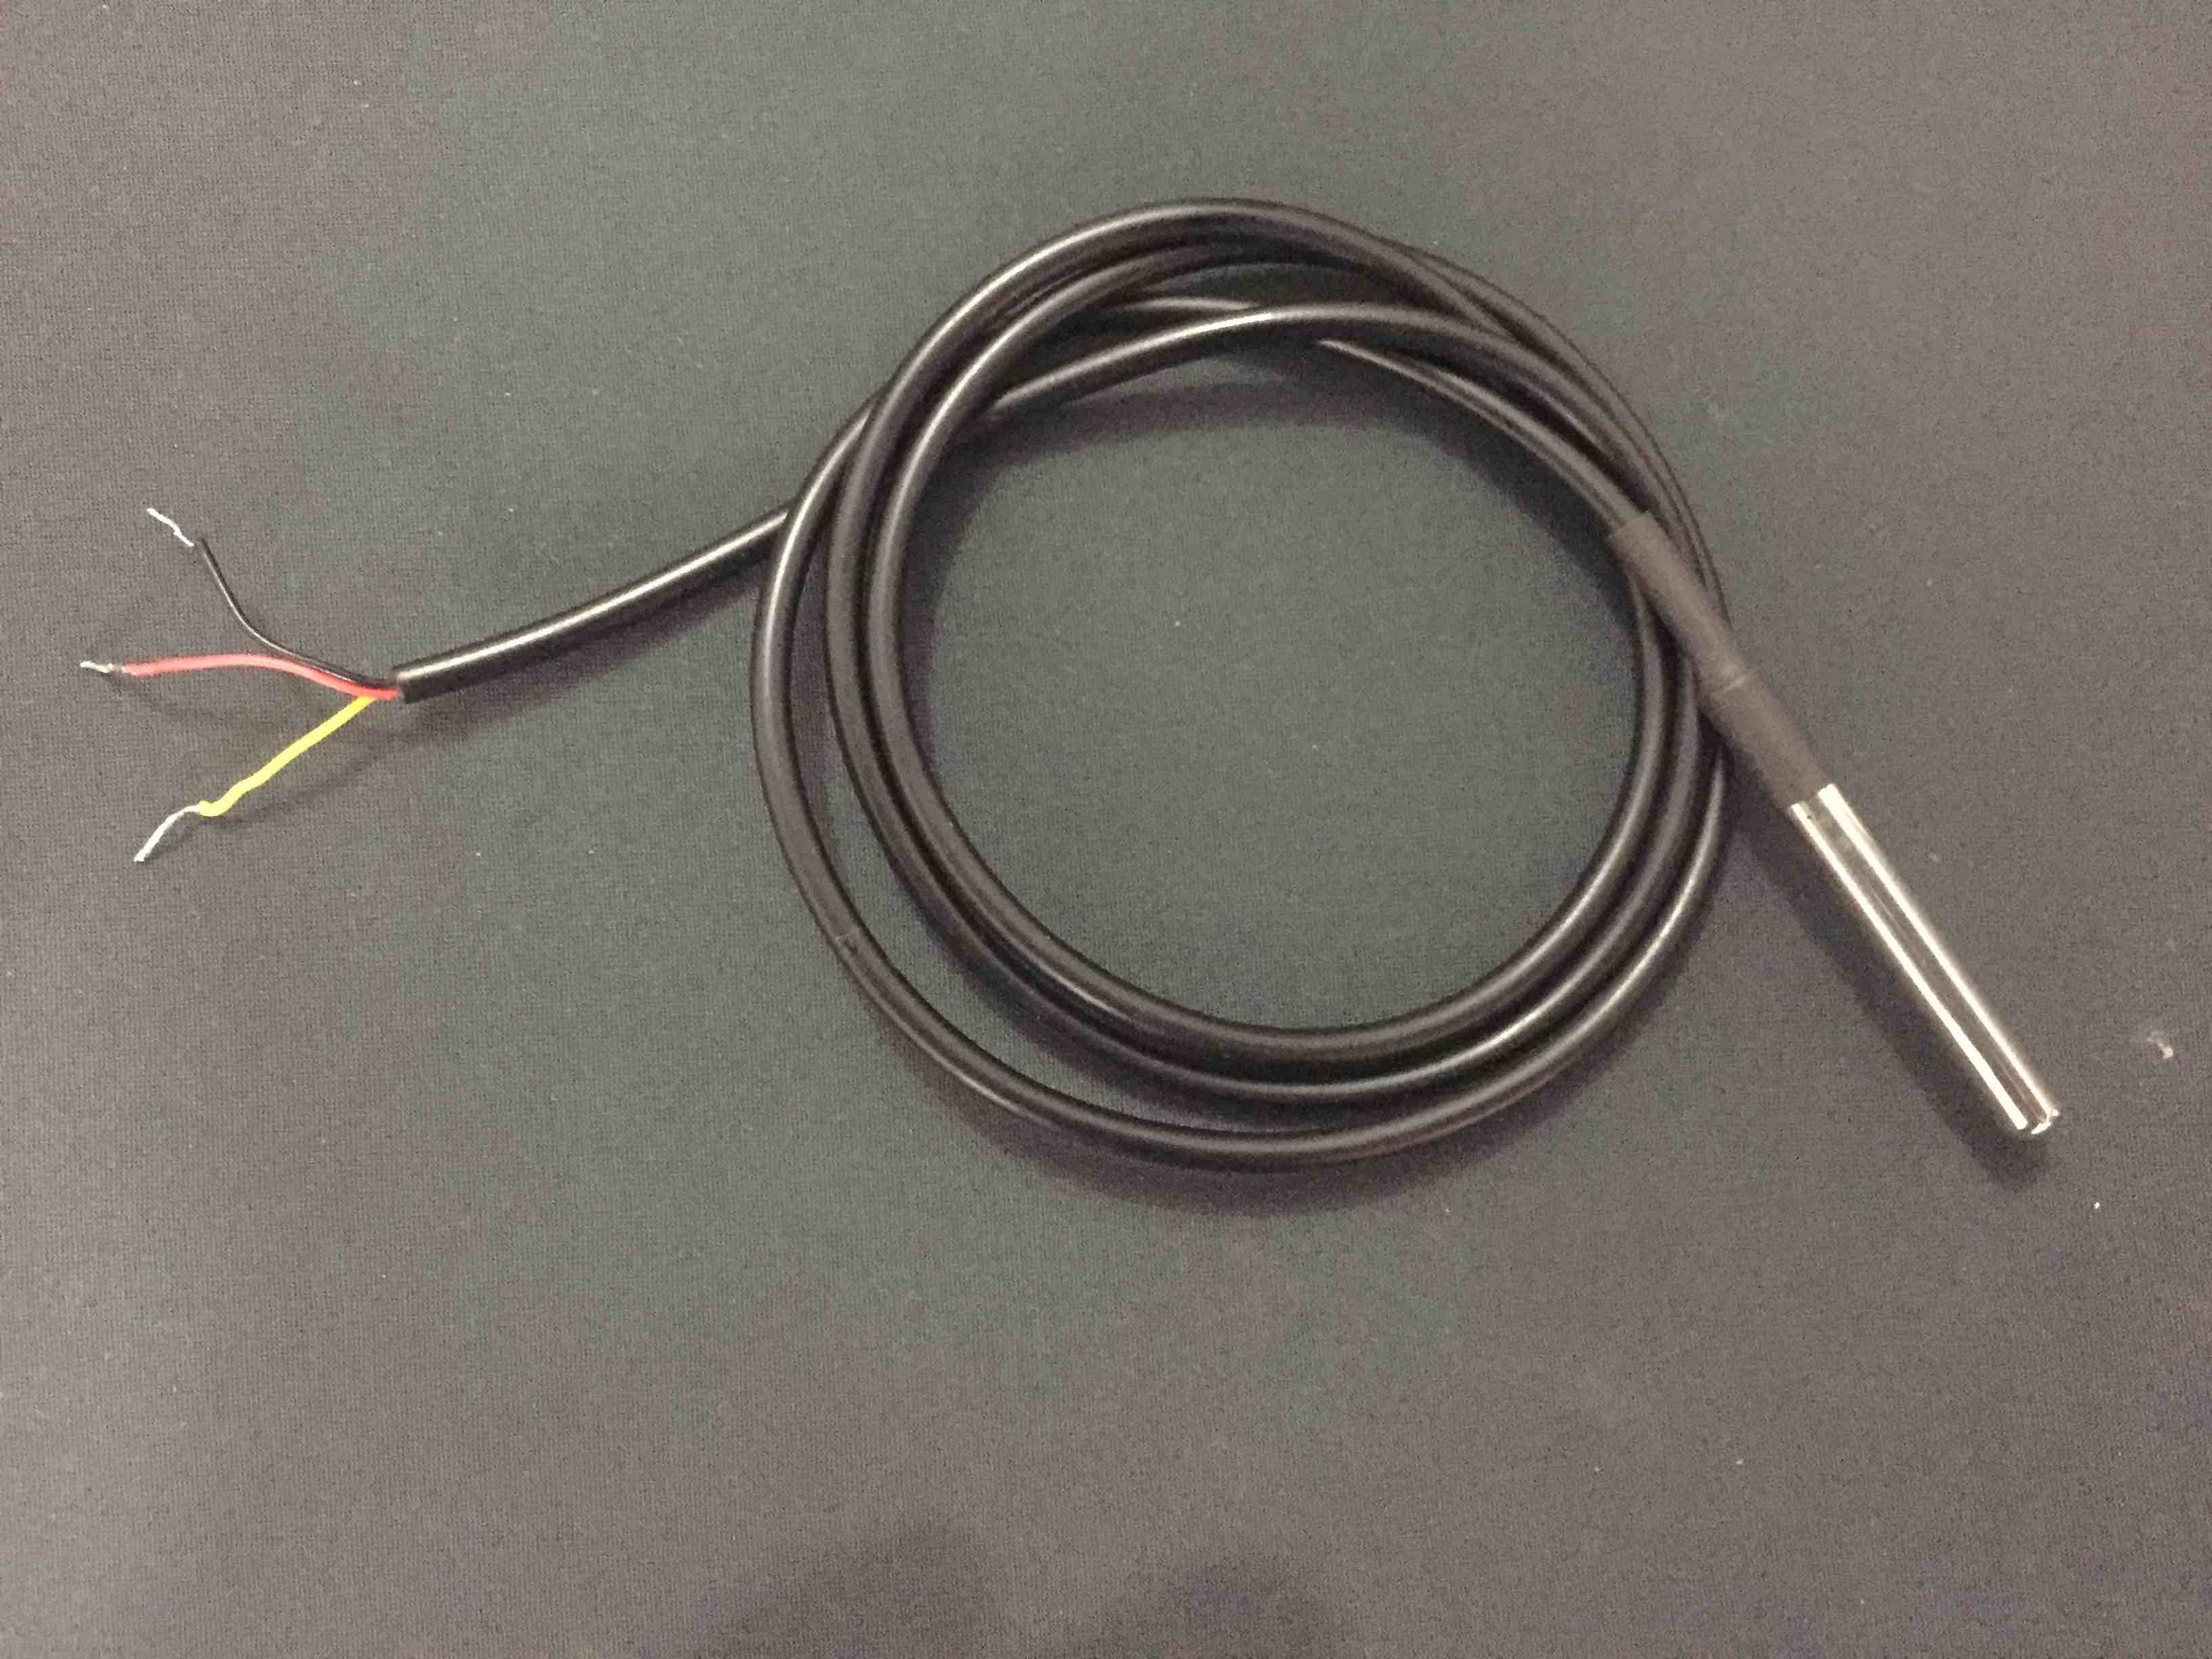
\includegraphics[scale= 0.08]{figuras/temperatura.jpg}
            \caption{Sensor de temperatura DS18B20. Fonte: Própria.}
            \label{sensor-temperatura}
\end{figure}
               
A medição da temperatura irá permitir a ativação do compressor mantendo a temperatura na faixa
ideal entre $-1$ e $1 ^\circ C$. Tal ativação será realizada pelo acionamento de um módulo relé  
ligado ao compressor. 
    
\begin{figure}[!htb]
           \centering
           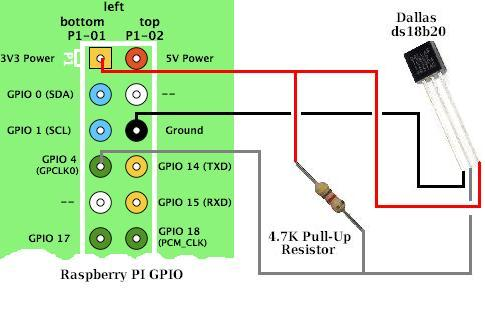
\includegraphics[scale= 0.5]{figuras/esquema.jpg}
            \caption{Esquemático do sensor de temperatura. Imagem da internet.}
            \label{esquema-temperatura}
\end{figure}    
    

\subsection{Controle de saída de chopp}

\subsubsection{Presença do copo}
Há a necessidade de se verificar a presença do copo no sistema para que o chopp possa ser tirado. 
Para tanto, inicialmente utilizou-se o sensor ultrassônico HC-SR04, porém, o mesmo inviabilizou seu
uso devido a complexidade de sua comunicação com o computador (\textit{Raspberry pi}).

Como solução mais direta e que evitaria tal nível de complexidade, optou-se por utilizar um sensor de trilha, 
que se comunica de forma direta com o computador e retorna um valor binário para a presença ou não do copo. 
Essa escolha traz como consequências, a necessidade de uma tira branca no copo
(sendo a mesma posicionada embaixo do copo) e a necessidade de uso de um copo transparente, para não
interferir com os sensores.


\subsubsection{Controle de fluxo}
Para que se pudesse ter um controle do volume presente no copo e consequentemente volume 
restante nos reservatórios inicialmente pensou-se em utilizar dois sensores (por redundância), 
sendo eles o sensor de fluxo YFS201 e uma célula de carga.

Obtiveram-se resultados satisfatórios na montagem do sensor de fluxo, porém verificou-se um erro 
muito grande em suas medidas, o qual chegava a dez porcento nos testes efetuados. 
Já quanto ao sensor de carga, não houve sucesso em sua implementação, apresentando resultados quase que aleatórios.

Após discutir o presente problema com professores e orientadores, outra solução foi proposta.
A solução proposta se utiliza de diodos emissores de luz e fototransistores posicionados a 
uma distância conhecida. Sabendo-se a bitola do tubo utilizado e, contando-se o tempo entre 
os acionamentos, pode-se calcular o fluxo passante, porém também não se obteve sucesso nessa abordagem

A solução final encontrada foi se utilizar de sensores de trilha posicionados ao longo do copo, juntamente com um acionamento 
por tempo. O acionamento por tempo garante que não se passe do volume total do copo, em caso de falha,
e o sensores de trilha garantem o volume solicitado. Isso foi projetado de modo que se garantisse uma maior precisão e eficácia
na tiragem do chopp, dadas pelos sistemas redundantes.


\subsubsection{Controle de colarinho}
O controle do colarinho é feito através da atuação de motores, estes que irão movimentar
a alavanca que controla a saída de chopp e colarinho. Desta forma é necessário realizar 
medições de tempo para cada tamanho de colarinho selecionável, servindo assim a quantidade. 
Esse acionamento é feito por tempo e relaciona-se com a entrada de ar no  sistema.


\subsection{Atuação dos motores}
Dois dos mais importantes subsistemas que contribuem diretamente com a experiência do usuário são 
a inclinação do copo e a tiragem automática do chopp, para tais tarefas fez-se o uso de motores de passo.
Para o controle dos motores usou-se dos pinos da \textit{Raspberry pi}, o uso dessa plataforma é necessário 
devido ao fato de que as bobinas dos motores devem funcionar constantemente,
para não interrupção do serviço,optou-se pelo o uso da mesma.

Os motores são alimentação com uma de 12V, para isso usou-se uma fonte de energia externa, 
devido ao consumo de corrente dos motores ser superiores ao que se pode fornecer com o microcontrolador, 
fez-se necessário o uso de um \textit{driver} L298N. A Figura \ref{motor} mostra o sistema dos motores montado.

\begin{figure}[!h]
            \centering
         	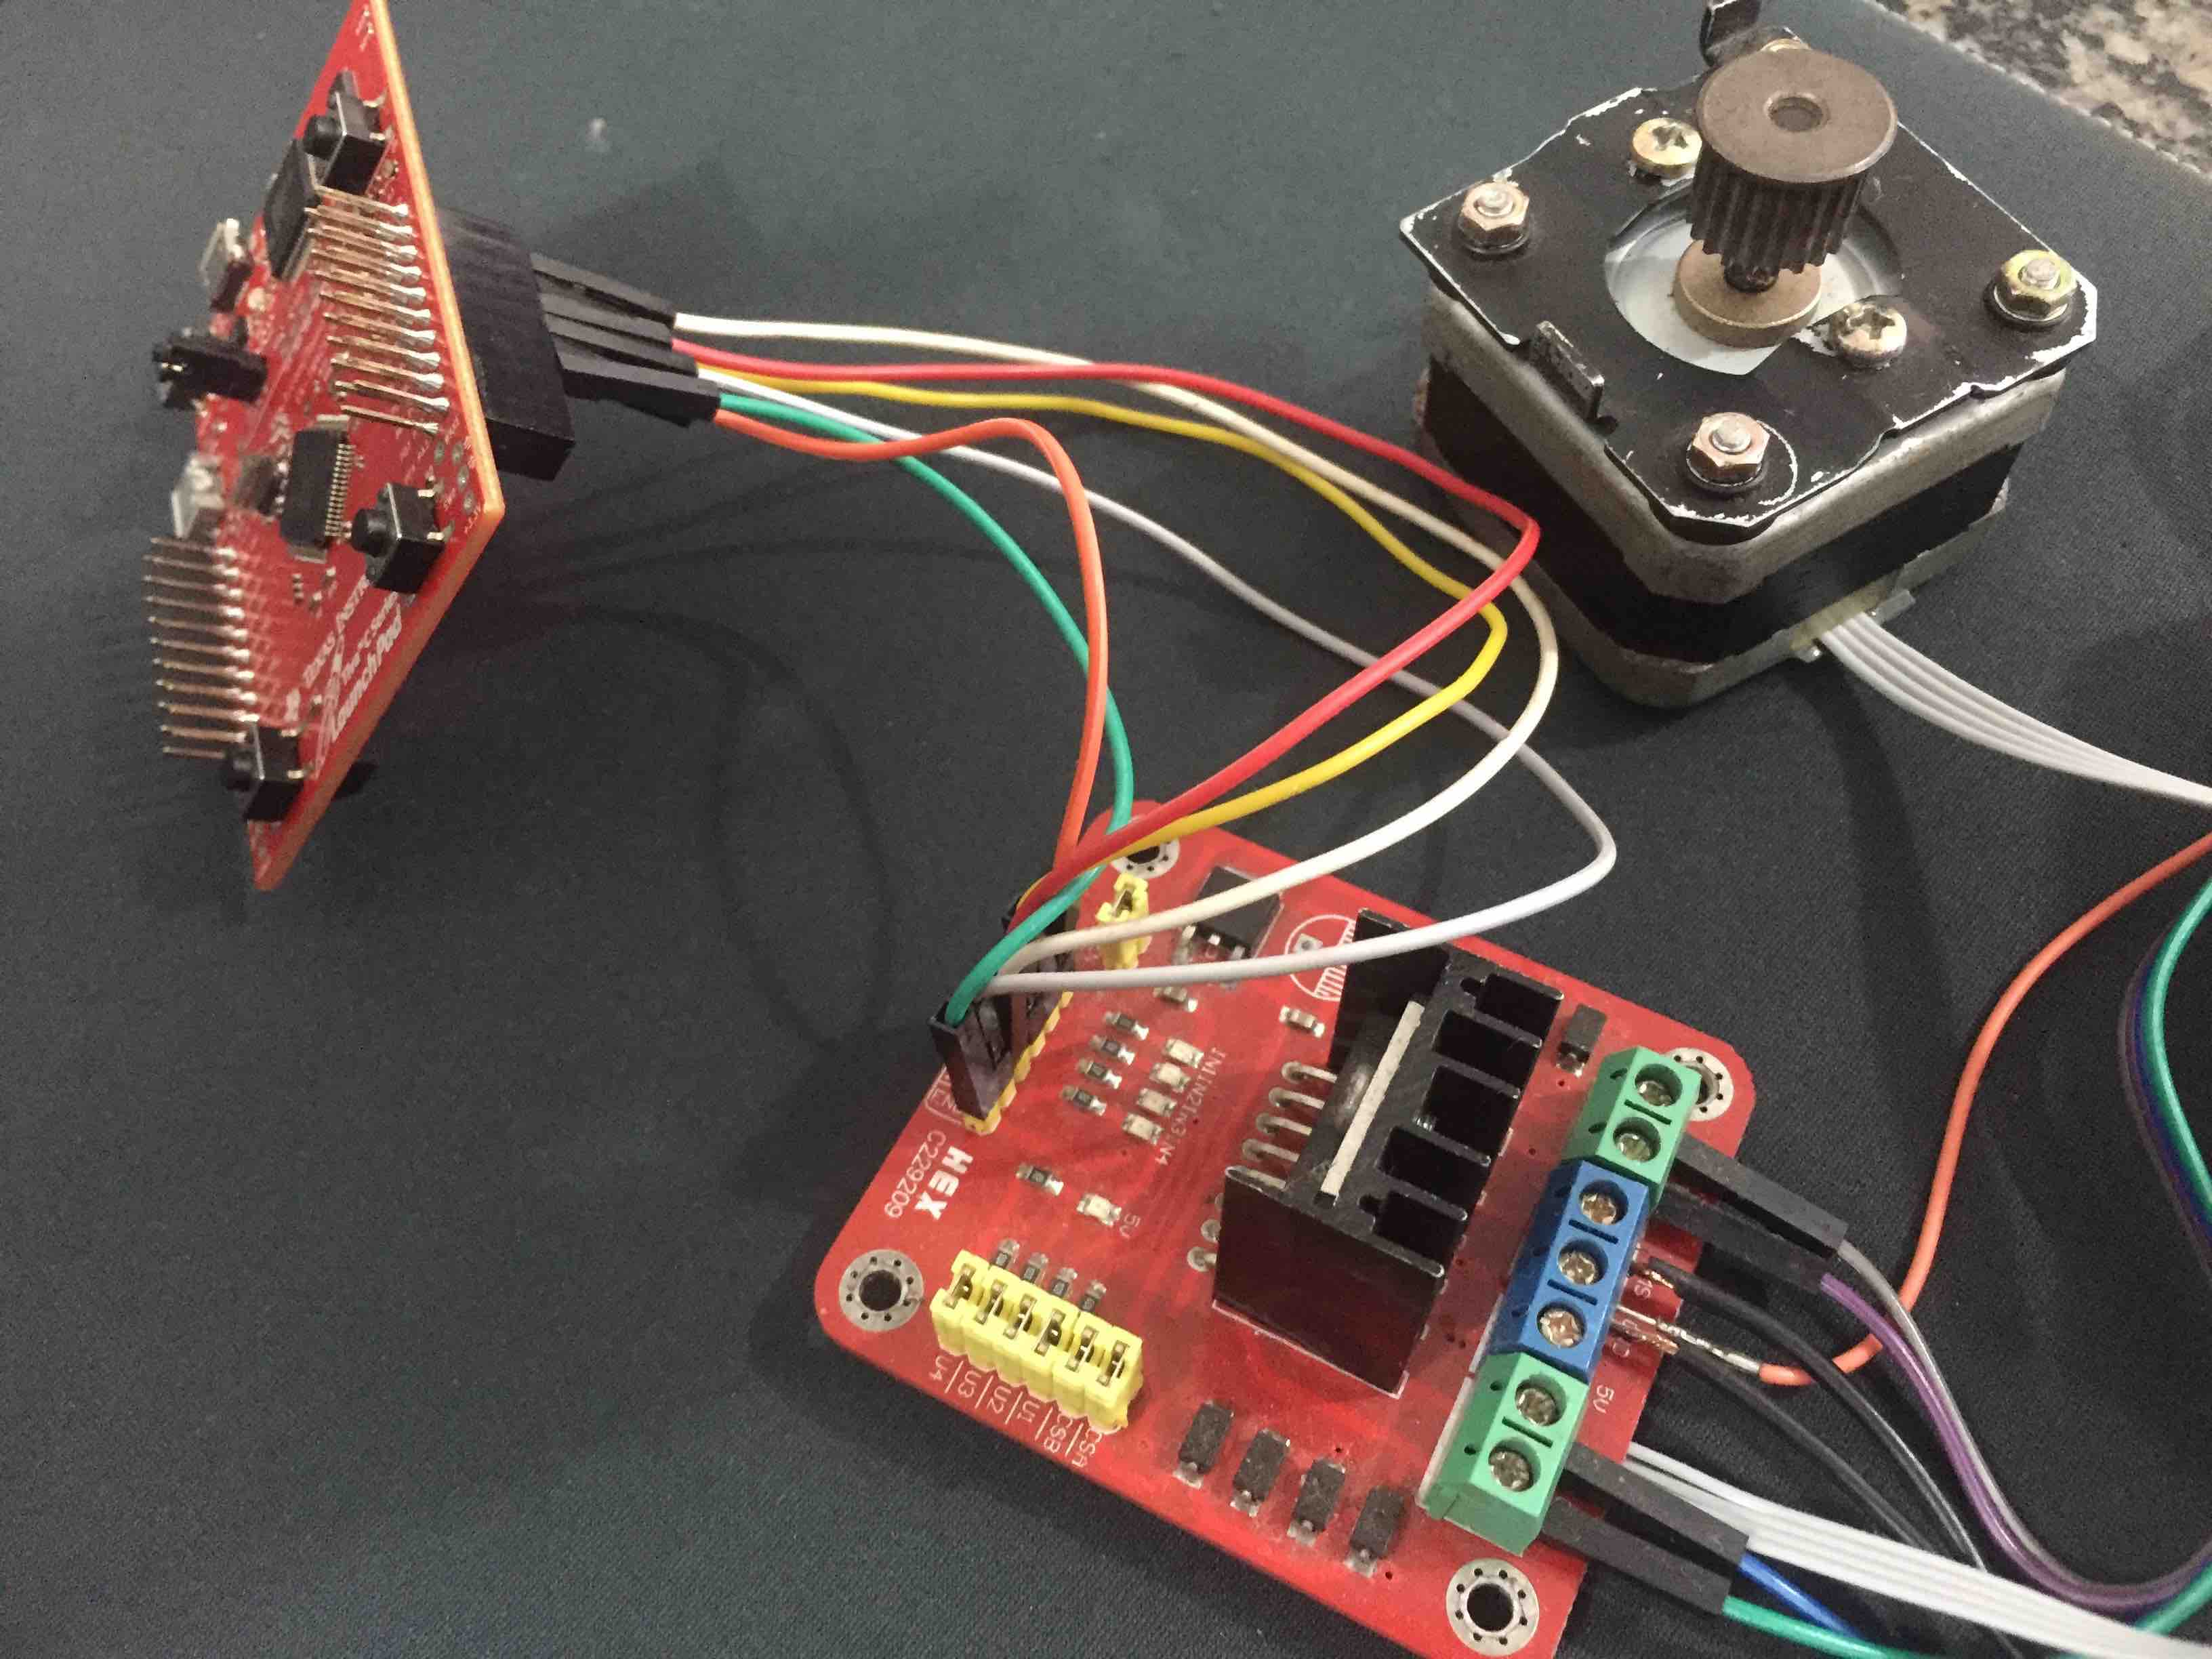
\includegraphics[scale= 0.08]{figuras/motor.jpg}
            \caption{Sistema de acionamento de motor de passo.}
            \label{motor}
\end{figure}

\newpage
\subsection{Abertura do reservatório de copos}

 Esse serviço se fez necessário, após a decisão de disponibilizar o copo ao usuário, 
 portanto os copos devem ser armazenados na própria máquina. Para disponibilizar os copos, 
 eles estarão dispostos de forma que sempre que exista uma requisição de um chopp, 
 um copo caia em um reservatório próprio. Para empurrar os copos são utilizados duas 
 solenoides de modelo TAU-0530, que pode ser visto na Figura \ref{solenoide}. 

\begin{figure}[!h]
            \centering
         	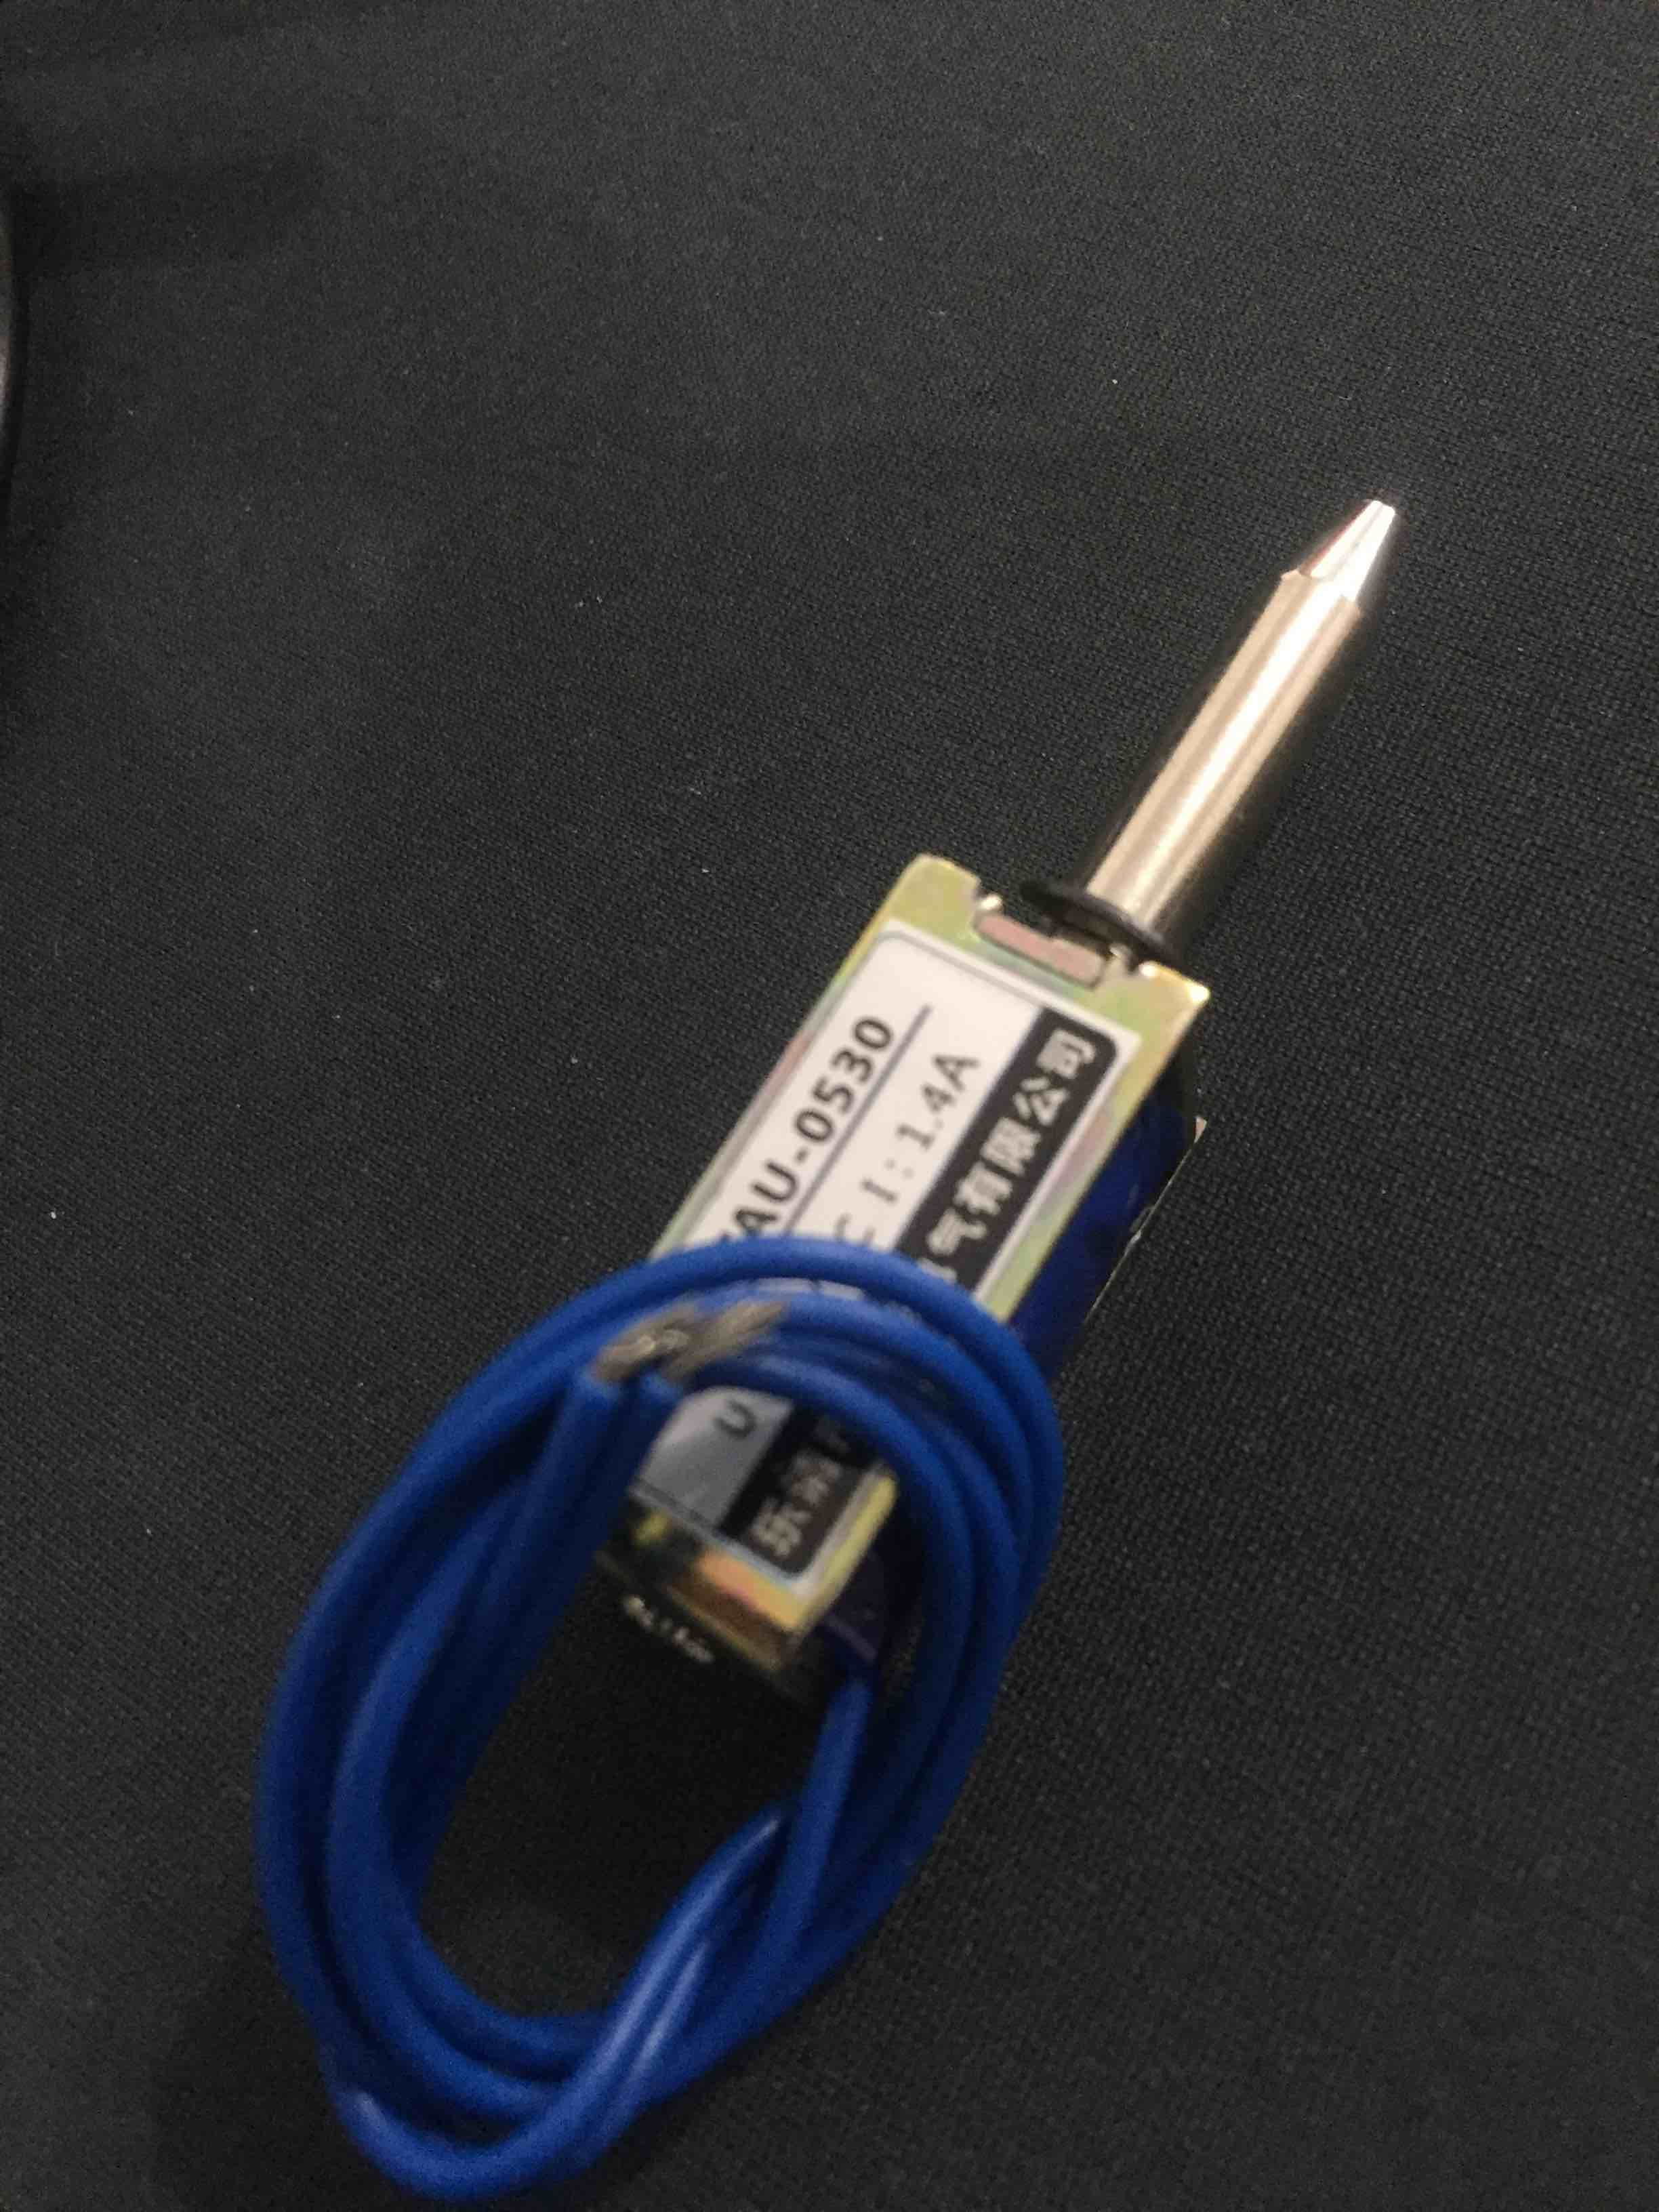
\includegraphics[scale= 0.06]{figuras/solenoide.jpg}
            \caption{Solenoide utilizado.}
            \label{solenoide}
\end{figure}

	
\section{Relatório de teste}



